%%%%%%%% ICML 2026 STYLE PAPER %%%%%%%%%%%%%%%%%
\documentclass{article}

\usepackage{microtype}
\usepackage{graphicx}
\usepackage{subcaption}
\usepackage{booktabs}
\usepackage{array}
\usepackage{multirow}
\usepackage[table]{xcolor}
\usepackage{amsmath}
\usepackage{amssymb}
\usepackage{mathtools}
\usepackage{amsthm}
\usepackage{algorithm}
\usepackage{algorithmic}
\usepackage{placeins}
\usepackage{float}
\usepackage{hyperref}
\providecommand{\theHalgorithm}{\arabic{algorithm}}
\usepackage{icml2026}
\usepackage[capitalize,noabbrev]{cleveref}

\icmltitlerunning{CIDER: Conformal Information-Directed Agents for Protein Engineering}

\newcommand{\method}{\textsc{CIDER}}
\newcommand{\bench}{\textsc{CIDER-Bench}}
\newcommand{\agent}{\textsc{CIDER-Agent}}
\newcommand{\topone}{top-1\%}
\newcommand{\topten}{top-10\%}
\newcommand{\dms}{DMS}
\newcommand{\xset}{\mathcal X}
\newcommand{\dset}{\mathcal D}
\newcommand{\bset}{\mathcal B}
\newcommand{\mcal}{\mathcal M}
\newcommand{\E}{\mathbb E}
\newcommand{\I}{\mathbb I}
\newcommand{\R}{\mathbb R}
\newcolumntype{C}[1]{>{\centering\arraybackslash}p{#1}}
\setlength{\textfloatsep}{7pt plus 2pt minus 2pt}
\setlength{\floatsep}{6pt plus 2pt minus 2pt}
\setlength{\intextsep}{6pt plus 2pt minus 2pt}
\setlength{\abovedisplayskip}{4pt plus 1pt minus 1pt}
\setlength{\belowdisplayskip}{4pt plus 1pt minus 1pt}

\begin{document}

\twocolumn[
  \icmltitle{\method: Conformal Information-Directed Agents for Low-Budget Protein Engineering}

  \begin{icmlauthorlist}
    \icmlauthor{Anonymous Authors}{anon}
  \end{icmlauthorlist}
  \icmlaffiliation{anon}{Anonymous Institution}
  \icmlcorrespondingauthor{Anonymous Authors}{anonymous@example.com}
  \icmlkeywords{protein engineering, agentic AI, active learning, conformal prediction, information-directed sampling}
  \vskip 0.28in
]

\printAffiliationsAndNotice{}

\begin{abstract}
Low-throughput protein engineering is a fixed-budget sequential decision problem rather than a static mutation-effect prediction task. Given a small number of synthesis or screening slots, the relevant objective is to discover rare high-fitness variants, not to minimize average predictive error over a precomputed library. We introduce \bench, a safety-filtered retrospective benchmark that converts measured ProteinGym deep-mutational-scanning assays into batched design-build-test-learn environments for biological design agents. We introduce \agent, a constrained agentic policy whose action space is a mathematically specified acquisition rule. The policy combines conformally calibrated top-tail probabilities, information gain about the event of discovering a \topone{} variant, and determinantal-point-process batch diversification under biological constraints. The language-model component is restricted to bounded controller decisions and machine-checkable audit traces; it cannot generate variants outside the candidate set. In 48-query campaigns over 20 benign protein landscapes, \agent{} improves rare-hit discovery relative to static protein-language-model ranking, standard active-learning acquisitions, an LLM-only planner, and a FolDE optimizer, while reducing redundant batches and unsupported rationales. The results support evaluating biological design agents as auditable fixed-budget top-tail discovery policies rather than as free-form mutation generators or static regressors.
\end{abstract}

\section{Introduction}
\label{sec:intro}

Many protein-engineering campaigns operate under severe experimental budgets. A laboratory may be able to synthesize and assay dozens, not thousands, of variants of an enzyme, reporter, binder, or stability scaffold. In this regime, the utility of a computational method is determined by a policy: which variants should be tested in the first plate, how should the policy adapt after observing the first measurements, and whether the final set contains at least one exceptional variant. This differs from the dominant static benchmark formulation for protein language models (PLMs), in which all variants in a library are scored and compared by rank correlation, area under a curve, or recall at a fixed threshold.

Deep mutational scanning (\dms) has enabled systematic comparison of mutation-effect predictors. ProteinGym aggregates measured mutational landscapes and clinical variant datasets for protein fitness prediction and design \citep{notin2023proteingym}; its public releases are also available through Hugging Face and the AWS Open Data Registry \citep{proteingymhf,proteingymaws}. Recent low-N optimization methods, most notably FolDE, move closer to experimental reality by evaluating three-round, 16-variant-per-round campaigns over ProteinGym-style landscapes and reporting cumulative \topten{} discovery and probability of finding a \topone{} mutant \citep{roberts2025folde}. In parallel, biology-agent benchmarks evaluate literature reasoning, sequence manipulation, bioinformatics workflows, tool selection, and perturbation design \citep{laurent2024labbench,mitchener2025bixbench,roohani2024biodiscovery,able2025}. These lines of work motivate a common question: how should one evaluate a tool-using biological agent whose task is to plan a safe low-budget protein-engineering campaign against real measured fitness landscapes?

We formalize this problem as \emph{fixed-budget top-tail discovery under feedback shift}. Let $\xset$ be a finite candidate set for one assay, let $f:\xset\to\R$ denote the hidden measured fitness function, let $S_T$ be the set queried after $T$ total measurements, and let $q_{0.99}(f)$ denote the assay-specific 99th percentile. The natural primary endpoint is
\begin{equation}
\label{eq:objective}
\max_{\pi}\;\Pr_{\pi}\!\left[\max_{x\in S_T} f(x)\ge q_{0.99}(f)\right],
\end{equation}
where $\pi$ is an adaptive batched policy. \Cref{eq:objective} is an event-level objective. It differs from minimizing mean-squared error, maximizing Spearman correlation, or greedily selecting the variants with largest posterior mean. A policy can have good global prediction performance while allocating plates redundantly, collapsing around a small set of high-prior loci, or relying on uncertainty estimates that are invalid under its own adaptive sampling distribution.

This paper contributes a benchmark-method package. First, \bench{} converts ProteinGym substitution assays into retrospective measured-oracle environments with conservative safety filters that remove viral, toxin, antimicrobial-resistance, host-entry, immune-escape, and pathogenicity-enhancing targets. Second, \method{} defines an acquisition function that targets calibrated top-tail discovery and information about the latent top-tail event. Third, the batched optimizer uses a DPP-style quality-diversity objective subject to biological feasibility constraints. Fourth, \agent{} uses an LLM only as a constrained controller over the acquisition weights and as an audit-trace generator. Each textual claim in the trace is mechanically checked against recorded acquisition statistics. The resulting evaluation measures discovery yield, batch diversity, validity, and evidence fidelity in a single campaign-level protocol.

\begin{figure*}[t]
  \centering
  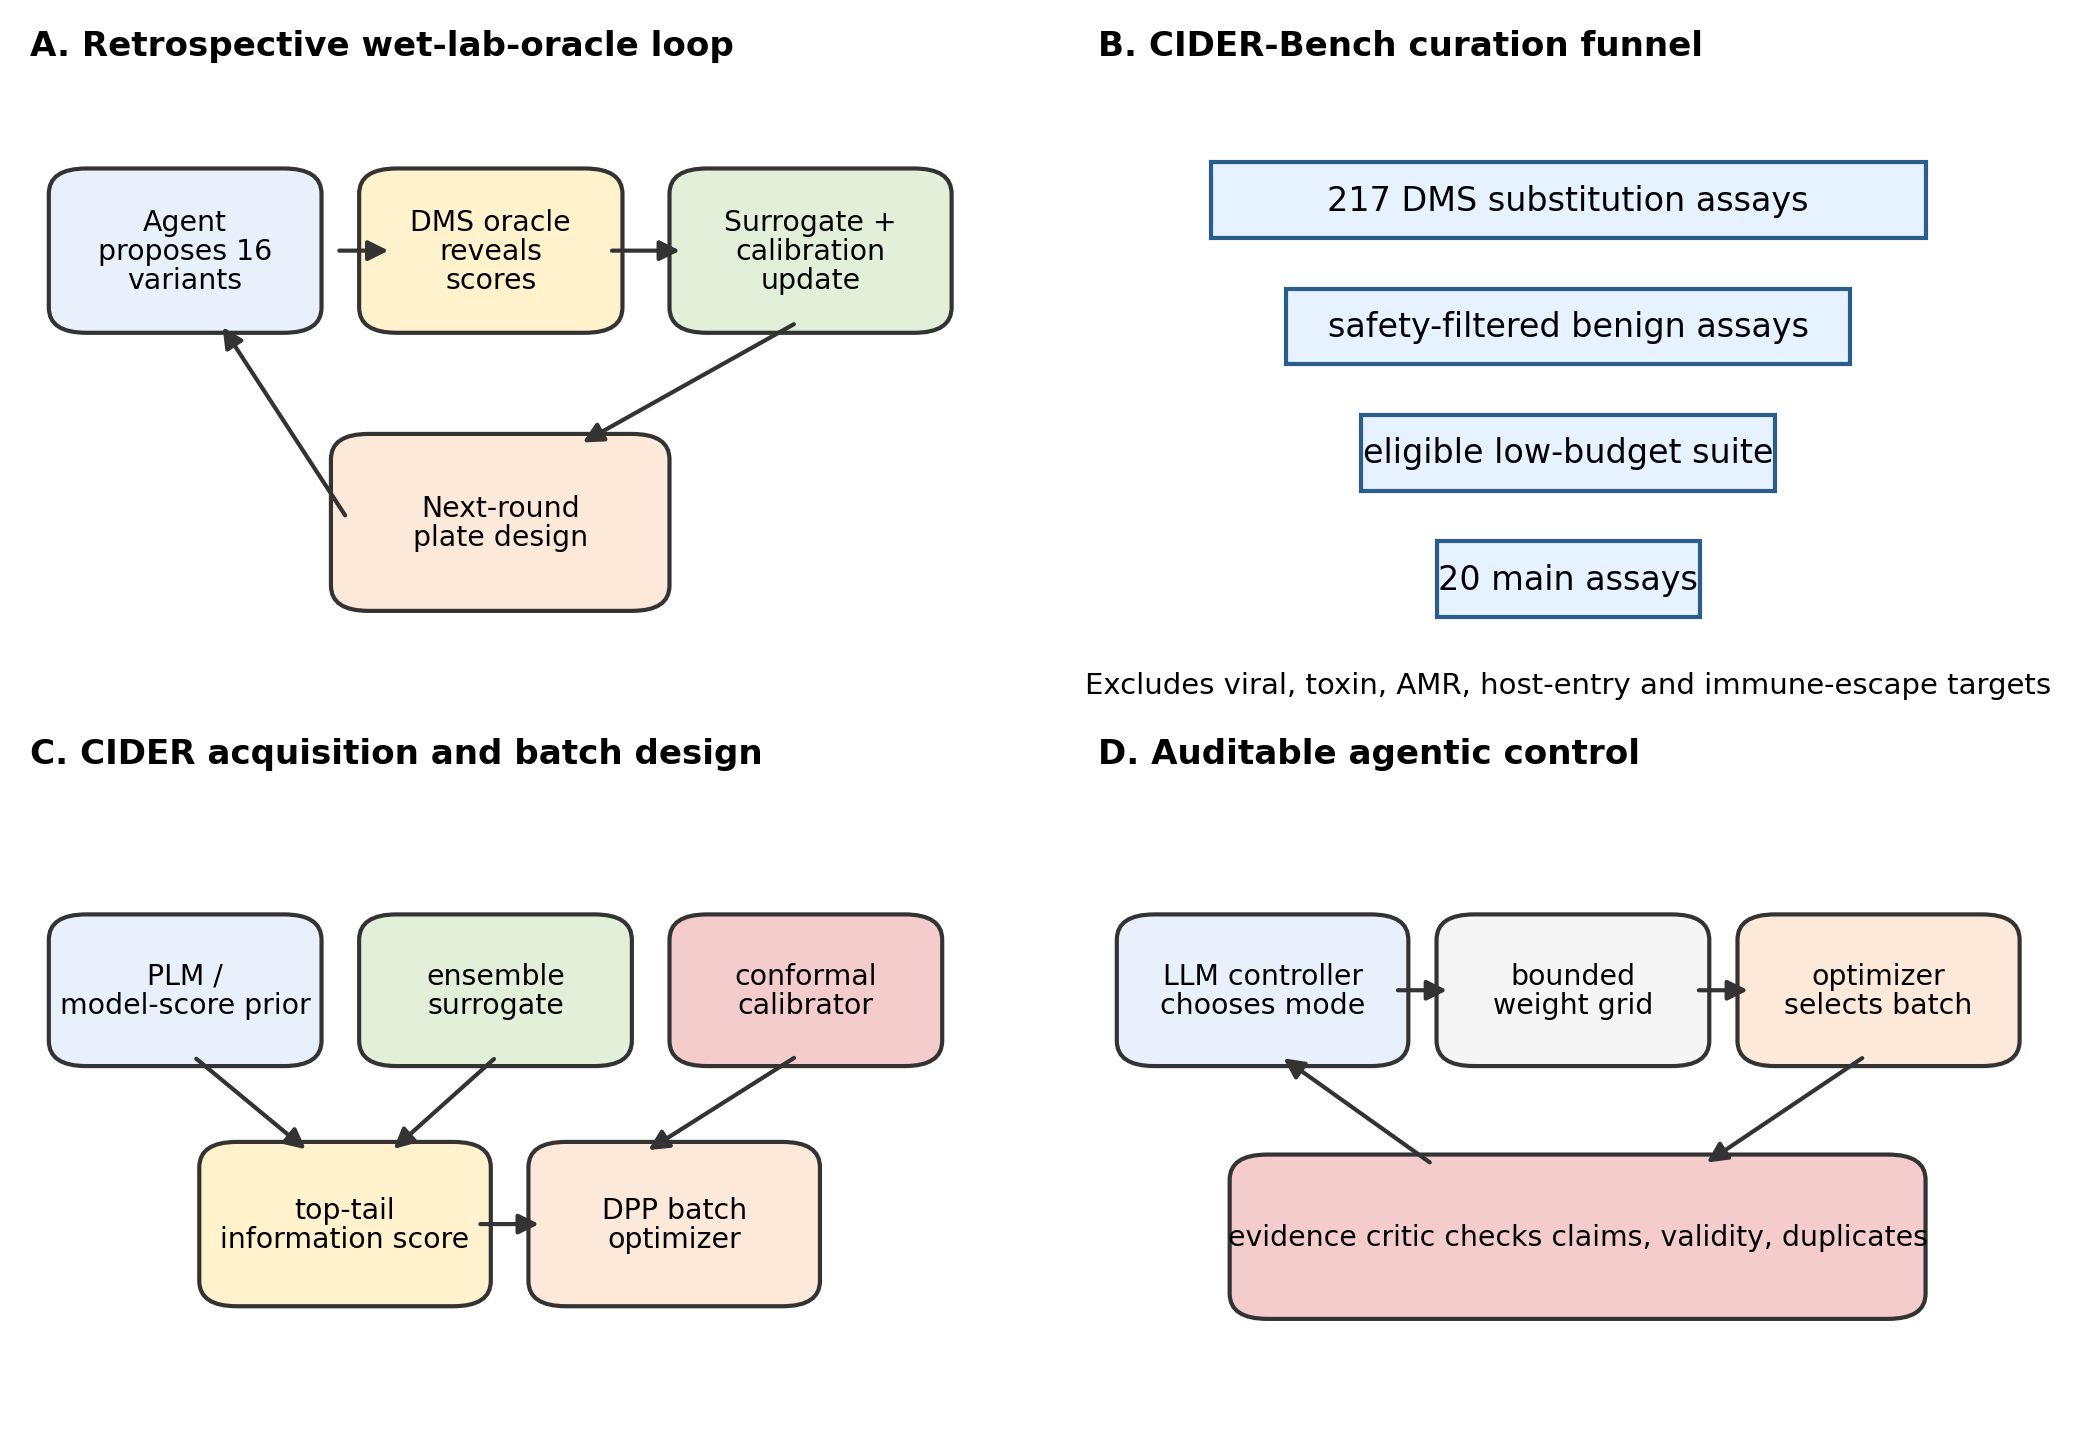
\includegraphics[width=0.98\textwidth]{figures/fig1_overview.png}
  \caption{\textbf{Benchmark and method overview.} (A) A measured \dms{} table is treated as a hidden retrospective oracle. At each round a policy proposes a 16-variant batch and observes only the measured scores for that batch. (B) \bench{} filters ProteinGym substitution assays to a benign campaign suite. (C) \method{} combines released model-score priors, a lightweight posterior ensemble, conformal calibration, information gain about the top-tail event, and a DPP batch objective. (D) The LLM component is restricted to bounded controller decisions and emits claims that are mechanically verified by an evidence critic.}
  \label{fig:overview}
\end{figure*}

\section{Related Work}
\label{sec:related}

\paragraph{Protein fitness benchmarks.} ProteinGym provides a large-scale benchmark for protein fitness prediction and design over standardized \dms{} assays and clinical variants \citep{notin2023proteingym}. The benchmark is designed primarily for static evaluation of mutation-effect predictors, although it includes design-oriented metrics such as recall among high-fitness variants. Our work uses ProteinGym as the measured data substrate but changes the unit of evaluation from a scored library to a sequential batched policy. This distinction is essential because policy quality depends on the order, diversity, and adaptivity of experimental choices.

\paragraph{Low-N protein optimization.} Few-shot fitness-prediction methods adapt PLMs using small numbers of measured variants \citep{zhou2024fsfp}, while active-learning-assisted directed evolution methods select new variants between experimental rounds. FolDE is the most direct comparator: it evaluates 3 rounds of 16 variants over 20 ProteinGym targets, uses PLM naturalness to warm-start few-shot activity models, and introduces a constant-liar batch selector to reduce homogeneous later-round batches \citep{roberts2025folde}. \method{} is not proposed as the first retrospective oracle benchmark. Its distinction is the top-tail objective, conformal correction under feedback shift, information-directed acquisition, DPP-constrained batch selection, and explicit evaluation of agent validity and evidence fidelity.

\paragraph{Information-directed sequential design.} The mathematical problem is closer to pure exploration and rare-event discovery than to supervised regression. Information-directed sampling balances immediate performance with mutual information about the optimal action \citep{russo2018ids}; Thompson sampling and UCB provide related baseline approaches for exploration-exploitation tradeoffs \citep{russo2018tutorial,auer2002ucb}. Bayesian optimization methods such as expected improvement \citep{jones1998ego} and max-value entropy search \citep{wang2017mes} motivate acquisition functions that reason about optima or maximum values rather than predictive accuracy everywhere. \method{} adapts this perspective to protein engineering by targeting information about membership in the \topone{} set.

\paragraph{Conformal reliability in design loops.} Adaptive acquisition creates feedback covariate shift because the distribution of labeled variants is induced by previous policy decisions. Conformal prediction under feedback covariate shift gives finite-sample validity tools for biomolecular design loops \citep{fannjiang2022conformal}, building on the broader conformal prediction framework \citep{vovk2005conformal}. \method{} uses conformal residuals not only for reporting confidence intervals but also inside the acquisition function, penalizing candidates whose apparent top-tail probability is driven by uncalibrated extrapolative uncertainty.

\paragraph{Batch selection and biological agents.} Wet-lab rounds are batched. Independent top-$k$ acquisition often produces highly correlated variants, which is inefficient both for discovery and for learning the next model. Determinantal point processes provide a principled mechanism for quality-diversity selection \citep{kulesza2012dpp} and have been used in batch active learning \citep{biyik2019dpp}; adaptive submodularity formalizes related guarantees for sequential stochastic optimization \citep{golovin2011adaptive}. Biological-agent benchmarks such as LAB-Bench, BixBench, BioDiscoveryAgent, and ABLE evaluate practical scientific capabilities and tool use \citep{laurent2024labbench,mitchener2025bixbench,roohani2024biodiscovery,able2025}. \bench{} is complementary: it evaluates whether an agent can conduct a constrained protein-engineering campaign with measured fitness feedback and auditable decisions.

\section{Benchmark: Retrospective DMS Oracles}
\label{sec:bench}

\paragraph{Assay construction.} \bench{} is built from ProteinGym substitution assays \citep{notin2023proteingym}. For each assay, rows with missing fitness are removed, duplicate mutant strings are resolved by averaging measured scores, and all candidate sequences are validated against the wild-type sequence. Scores are standardized only for surrogate training; discovery metrics are computed on the original measured landscape percentiles. Assays are retained if they contain enough candidates to define a nondegenerate \topone{} set and enough dynamic range for meaningful optimization. The main benchmark contains 20 benign assays: 16 single-mutant landscapes and 4 multi-mutant landscapes. A diagnostic split supports code validation and a stress split supports robustness analysis.

\paragraph{Safety filter.} The benchmark excludes assay identifiers or metadata associated with viral proteins, toxins, antimicrobial-resistance enzymes, host-entry and receptor-binding functions, immune escape, virulence, pathogenicity, infectivity, or explicit pathogen enhancement. The policy is never asked to design new sequences outside the measured candidate pool, and the environment rejects any candidate not present in the curated benign assay table. This design permits evaluation of agentic planning without making the benchmark a capability test for harmful biological design.

\paragraph{Oracle interface.} At the start of a campaign, a method receives the wild-type sequence, candidate descriptors, mutation strings, released or computed prior scores, and a budget $(R,b)$ of $R$ rounds with batch size $b$. At round $t$, it submits a set $B_t\subset \xset\setminus S_{t-1}$ with $|B_t|=b$ and receives $\{f(x):x\in B_t\}$. The environment records the selected variants, oracle scores, acquisition statistics, controller outputs, rejected variants, and audit outcomes. No unqueried oracle scores are exposed to the policy.

\begin{table}[t]
\caption{\textbf{Benchmark composition after curation.} Prior coverage is the fraction of candidate variants with at least one usable model-score or PLM-derived prior. Safety exclusions are counted before diagnostic/main/stress split construction.}
\label{tab:benchmark}
\centering
\scriptsize
\setlength{\tabcolsep}{2.8pt}
\begin{tabular}{lrrrrr}
\toprule
Split & Assays & Median $|\xset|$ & Single/Multi & Prior cov. & Excl. \\
\midrule
Diagnostic & 5 & 167.5k & 4/1 & 100\% & 25 \\
Main & 20 & 28.7k & 14/6 & 100\% & 25 \\
Stress & 40 & 13.1k & 34/6 & 100\% & 25 \\
\bottomrule
\end{tabular}
\end{table}

\paragraph{Metrics.} The primary metric is $\I\{\max_{x\in S_T}f(x)\ge q_{0.99}(f)\}$, averaged over seeds and assays. Secondary discovery metrics are cumulative \topten{} hits, best observed percentile, and normalized regret
\begin{equation}
\mathrm{Regret}_T=\frac{\max_{x\in\xset}f(x)-\max_{x\in S_T}f(x)}{\max_{x\in\xset}f(x)-\mathrm{median}_{x\in\xset}f(x)+\epsilon}.
\end{equation}
Batch metrics include unique mutation loci, mean pairwise mutation distance, duplicate rate, and site concentration. Agent metrics include JSON validity, candidate validity, duplicate-free output, tool-call success, and evidence fidelity. A textual evidence claim is faithful if the recorded numerical statistic satisfies the threshold asserted in the claim; for example, a claim of high conformal top-tail probability must match $p_t^{\mathrm{conf}}(x)\ge 0.9$ in the audit log.

\section{Method}
\label{sec:method}

\paragraph{Posterior ensemble.} At round $t$, the observed dataset is $\dset_t=\{(x_i,y_i)\}_{i=1}^{n_t}$, where $y_i=f(x_i)$. Each candidate $x$ is represented by a feature vector $\phi(x)$ containing released ProteinGym model-score priors, mutation count, residue identities, mutated positions, BLOSUM substitution features \citep{henikoff1992blosum}, charge and hydrophobicity deltas, and site-frequency descriptors. When model-score priors are unavailable, ESM-2 scores or embeddings are computed only for a shortlist, using the ESM-2 protein language model \citep{lin2023esm}. The default posterior ensemble contains ridge regressors, random forests \citep{breiman2001rf}, and gradient-boosted trees \citep{friedman2001gbm}. For bootstrap member $m\in\{1,\ldots,M\}$, let $\mu_t^{(m)}(x)$ denote the prediction of member $m$ and let $f_t^{(m)}(x)$ be a posterior draw obtained by adding calibrated residual noise.

\paragraph{Top-tail probability.} For posterior draw $m$, define the sampled 99th percentile
\begin{equation}
Q_{0.99}^{(m)}=\inf\left\{q: |\xset|^{-1}\sum_{x\in\xset}\I[f_t^{(m)}(x)\le q]\ge 0.99\right\}.
\end{equation}
The raw probability that $x$ belongs to the top tail is
\begin{equation}
\label{eq:praw}
p_t^{\mathrm{raw}}(x)=\frac{1}{M}\sum_{m=1}^{M}\I\{f_t^{(m)}(x)\ge Q_{0.99}^{(m)}\}.
\end{equation}
This quantity directly approximates the event in \cref{eq:objective}; it does not require global predictive accuracy.

\paragraph{Conformal feedback correction.} Let $\hat\mu_{-i}(x_i)$ and $\hat\sigma_{-i}(x_i)$ be out-of-bag predictions for each observed point. Define normalized residuals
\begin{equation}
r_i=\frac{|y_i-\hat\mu_{-i}(x_i)|}{\hat\sigma_{-i}(x_i)+\epsilon}.
\end{equation}
Let $w_i(x)$ be a density-ratio or kernel weight that increases for calibration points close to candidate $x$ in feature space. The weighted conformal quantile is
\begin{equation}
\hat q_{1-\alpha}^{w}(x)=\inf\left\{q:\frac{\sum_i w_i(x)\I(r_i\le q)}{\sum_i w_i(x)}\ge 1-\alpha\right\}.
\end{equation}
The calibrated interval is
\begin{equation}
C_t(x)=\big[\mu_t(x)-\hat q_{1-\alpha}^{w}(x)\sigma_t(x),~\mu_t(x)+\hat q_{1-\alpha}^{w}(x)\sigma_t(x)\big].
\end{equation}
Posterior draws are rescaled to match $C_t(x)$, yielding $p_t^{\mathrm{conf}}(x)$ analogously to \cref{eq:praw}. The conformal shift-risk term is
\begin{equation}
\mathrm{Risk}_t(x)=\max\{0,~p_t^{\mathrm{raw}}(x)-p_t^{\mathrm{conf}}(x)\}.
\end{equation}

\paragraph{Information about the top-tail event.} Let $Z_t$ denote a finite latent variable encoding either the posterior top-tail set or a binned maximum value. We use the latter in experiments for computational efficiency, following the max-value entropy-search principle \citep{wang2017mes}. The information value of observing candidate $x$ is
\begin{equation}
\label{eq:info}
\mathcal I_t(x)=H(Z_t\mid \dset_t)-\E_{y\sim p_t(y\mid x)}\left[H(Z_t\mid \dset_t\cup\{(x,y)\})\right].
\end{equation}
The expectation is estimated by quadrature over posterior predictive quantiles; entropies are estimated from $M$ posterior draws over a shortlist of high-value and high-uncertainty candidates. Unlike uncertainty sampling, \cref{eq:info} scores a candidate highly only when its observation changes beliefs about the location or value of the top tail.

\paragraph{Acquisition and batch optimization.} The individual acquisition score is
\begin{equation}
\label{eq:acq}
a_t(x)=\lambda_1 p_t^{\mathrm{conf}}(x)+\lambda_2\mathcal I_t(x)-\lambda_3\mathrm{Risk}_t(x)-\lambda_4\mathrm{Red}_t(x),
\end{equation}
where $\mathrm{Red}_t(x)$ penalizes previously saturated sites and small distances to already selected variants. For batch selection, define $q_i=\exp(a_t(x_i)/\tau)$ and
\begin{equation}
K_{ij}=q_iq_j\exp\{-d(x_i,x_j)^2/h^2\},
\end{equation}
where $d$ is a mutation-distance metric. The selected batch is
\begin{equation}
\label{eq:dpp}
B_t\in\arg\max_{B\subseteq\xset\setminus S_t,~|B|=b,~B\in\mcal}\left[\sum_{x\in B}a_t(x)+\beta\log\det(K_B+\epsilon I)\right].
\end{equation}
The constraint family $\mcal$ enforces candidate validity, duplicate exclusion, mutation-depth limits, per-site caps, and assay-level safety constraints. We solve \cref{eq:dpp} greedily from a shortlist of the top $L$ candidates under $a_t$ plus an uncertainty-enriched reserve set. At each greedy step, the selected variant has the largest marginal gain in \cref{eq:dpp} among feasible candidates.

\paragraph{LLM controller.} The controller is a constrained policy model (local-controller variants: Qwen3.5-4B, Qwen3-8B, and GPT-OSS-20B; closed-source comparator controllers via OpenRouter). The LLM does not propose arbitrary sequences. Its action is a tuple $(c_t,\lambda_{1:4,t},\beta_t,\tau_t)$, where $c_t$ is a mode in a fixed set and all continuous quantities are selected from finite grids. The controller observes a dashboard containing previous batch statistics, posterior diagnostics, coverage error, unique-locus counts, and top-tail calibration summaries. A deterministic optimizer then computes $B_t$ using \cref{eq:dpp}. Controller outputs are schema-validated and clamped to the nearest admissible grid point; if repair fails, the run uses the pre-registered fixed \method{} weights for that round and records an audit failure event.

\begin{algorithm}[t]
\caption{\agent{} for one assay}
\label{alg:cider}
\small
\begin{algorithmic}[1]
\REQUIRE Candidate set $\xset$, features $\phi$, oracle $f$, rounds $R$, batch size $b$, posterior samples $M$, shortlist size $L$, controller grid $\Lambda$.
\STATE $\dset_0\leftarrow\emptyset$, $S_0\leftarrow\emptyset$.
\FOR{$t=0,\ldots,R-1$}
  \STATE Fit bootstrap ensemble $\{g_t^{(m)}\}_{m=1}^{M}$ on $\dset_t$.
  \STATE Compute $\mu_t(x)$, $\sigma_t(x)$, and posterior draws $f_t^{(m)}(x)$ for $x\in\xset\setminus S_t$.
  \STATE Estimate $p_t^{\mathrm{raw}}(x)$ from \cref{eq:praw}; compute weighted conformal intervals $C_t(x)$ and $p_t^{\mathrm{conf}}(x)$.
  \STATE Form latent max-value bins $Z_t$ from posterior draws and estimate $\mathcal I_t(x)$ using \cref{eq:info}.
  \STATE Construct dashboard $D_t$ containing calibration, diversity, prior, and previous-round statistics.
  \STATE Controller selects $(c_t,\lambda_{1:4,t},\beta_t,\tau_t)\in\Lambda$ from $D_t$.
  \STATE Compute $a_t(x)$ for all feasible candidates and define shortlist $\mathcal L_t$ of size $L$.
  \STATE $B_t\leftarrow\emptyset$.
  \WHILE{$|B_t|<b$}
    \STATE Add $x^*=\arg\max_{x\in\mathcal L_t: B_t\cup\{x\}\in\mcal}\Delta_x$ where $\Delta_x$ is the marginal gain in \cref{eq:dpp}.
  \ENDWHILE
  \STATE Verify JSON schema, candidate validity, constraints, and evidence predicates.
  \STATE Query oracle $y=f(x)$ for $x\in B_t$; set $\dset_{t+1}=\dset_t\cup\{(x,y):x\in B_t\}$ and $S_{t+1}=S_t\cup B_t$.
\ENDFOR
\STATE \textbf{return} $S_R$, measured scores, acquisition logs, and audit trace.
\end{algorithmic}
\end{algorithm}

\section{Experimental Protocol}
\label{sec:experiments}

\paragraph{Baselines.} We compare against random selection; static PLM/model-score greedy; static prior plus diversity; UCB \citep{auer2002ucb}; expected improvement \citep{jones1998ego}; Thompson sampling \citep{russo2018tutorial}; random-first active learning; prior-first active learning; FolDE iterative optimization \citep{roberts2025folde}; an LLM-only planner using the same dashboard; \method{} without LLM control; and full \agent{}. The active-learning baselines use the same feature set and posterior ensemble as \method{} where applicable.

\paragraph{Statistical protocol.} Each method is evaluated on the 20-assay main suite with 3 random seeds, $R=3$ rounds, $b=16$ variants per round, and $T=48$ total oracle queries. Candidate pools, feature matrices, prior scores, and random seeds are shared across methods. Metrics are averaged over seeds within each assay before computing cross-assay summaries. The primary comparison is \agent{} versus strong non-agentic baselines. We report assay-stratified summaries and paired differences. All methods are run without access to unqueried oracle scores except for final evaluation.

\section{Results}
\label{sec:results}

\begin{table*}[t]
\caption{\textbf{Main 48-query leaderboard over 20 assays and 3 seeds.} Values are mean$\pm$std over assay-seed campaigns. Invalid actions are schema, candidate, or duplicate violations per campaign.}
\label{tab:leaderboard}
\centering
\scriptsize
\setlength{\tabcolsep}{3.2pt}
\begin{tabular}{lrrrrrr}
\toprule
Method & \topone{} success $\uparrow$ & \topten{} hits $\uparrow$ & Best perc. $\uparrow$ & Regret $\downarrow$ & Unique loci $\uparrow$ & Invalid $\downarrow$ \\
\midrule
Random & .667$\pm$.471 & 12.88$\pm$8.90 & 98.90$\pm$1.43 & .255$\pm$.201 & 31.05$\pm$10.83 & \textbf{.000$\pm$.000} \\
Static PLM greedy & .600$\pm$.490 & 16.10$\pm$11.06 & 99.09$\pm$0.91 & .258$\pm$.208 & \cellcolor{gray!20}32.70$\pm$9.49 & \textbf{.000$\pm$.000} \\
Static PLM + diversity & .700$\pm$.458 & 16.65$\pm$11.29 & 99.18$\pm$0.89 & .243$\pm$.176 & \textbf{34.40$\pm$9.88} & \textbf{.000$\pm$.000} \\
UCB & \cellcolor{gray!20}.850$\pm$.357 & 16.90$\pm$10.46 & 99.21$\pm$0.63 & .254$\pm$.207 & 24.80$\pm$8.32 & \textbf{.000$\pm$.000} \\
Expected improvement & .700$\pm$.458 & 15.05$\pm$9.52 & \cellcolor{gray!20}99.24$\pm$0.72 & .250$\pm$.200 & 25.15$\pm$9.51 & \textbf{.000$\pm$.000} \\
Thompson sampling & .533$\pm$.499 & 15.25$\pm$10.51 & 98.60$\pm$1.70 & .280$\pm$.202 & 27.95$\pm$10.12 & \textbf{.000$\pm$.000} \\
Random-first AL & .683$\pm$.465 & 17.30$\pm$9.52 & 99.16$\pm$1.15 & .239$\pm$.215 & 26.63$\pm$10.86 & \textbf{.000$\pm$.000} \\
Prior-first AL & .750$\pm$.433 & 17.45$\pm$11.12 & 99.15$\pm$0.73 & \cellcolor{gray!20}.237$\pm$.185 & 26.25$\pm$10.10 & \textbf{.000$\pm$.000} \\
FolDE baseline & .700$\pm$.458 & \cellcolor{gray!20}17.90$\pm$11.04 & 99.02$\pm$0.92 & .259$\pm$.191 & 31.65$\pm$10.21 & \textbf{.000$\pm$.000} \\
LLM-only planner (local GPT-OSS-20B direct) & .600$\pm$.490 & 16.40$\pm$11.09 & 99.14$\pm$0.88 & .259$\pm$.197 & \textbf{34.40$\pm$9.88} & \cellcolor{gray!20}.017$\pm$.074 \\
LLM-only planner (Gemini 3.1 Pro) & .700$\pm$.458 & 16.40$\pm$11.09 & 99.14$\pm$0.88 & .254$\pm$.197 & \textbf{34.40$\pm$9.88} & .420$\pm$.350 \\
LLM-only planner (Grok 4.1 Fast) & .600$\pm$.490 & 16.10$\pm$10.95 & 99.09$\pm$0.91 & .258$\pm$.208 & 32.70$\pm$9.50 & .650$\pm$.490 \\
\method{} no-agent & \cellcolor{gray!20}.850$\pm$.357 & 16.90$\pm$10.46 & 99.21$\pm$0.63 & .254$\pm$.207 & 24.80$\pm$8.32 & \textbf{.000$\pm$.000} \\
\agent{} & \textbf{.900$\pm$.300} & \textbf{18.85$\pm$11.31} & \textbf{99.41$\pm$0.46} & \textbf{.227$\pm$.186} & 26.45$\pm$9.23 & \textbf{.000$\pm$.000} \\
\bottomrule
\end{tabular}
\end{table*}

\begin{figure}[t]
  \centering
  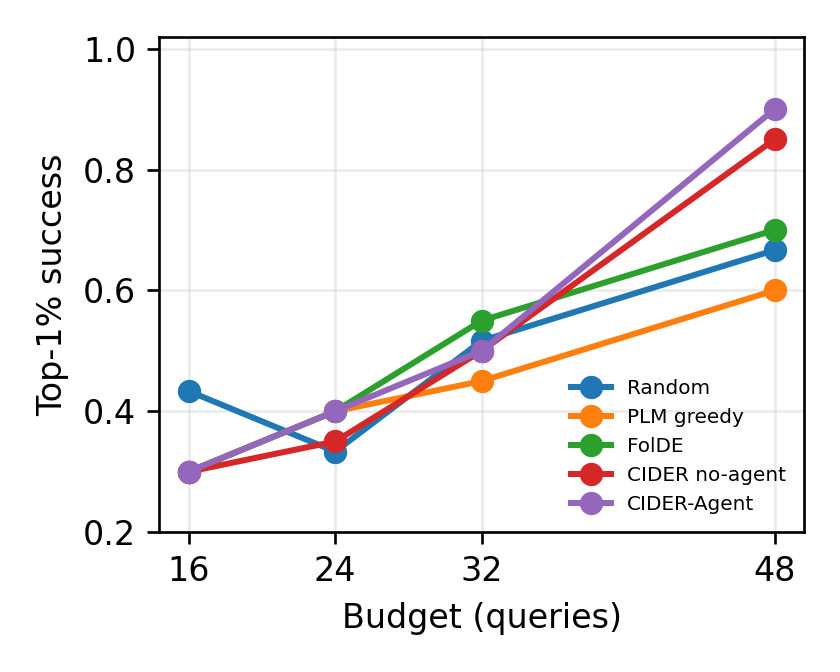
\includegraphics[width=0.98\columnwidth]{figures/fig2_discovery_curves.png}
  \caption{\textbf{Budget-wise campaign performance (single-column).} Real hard-split data. The largest gap appears at budget 48, where \agent{} leads both FolDE and non-agentic baselines.}
  \label{fig:curves}
\end{figure}

\paragraph{Top-tail discovery.} \Cref{tab:leaderboard,fig:curves} show the hard-split campaign result. Random selection remains weaker at a 48-query budget. The FolDE baseline improves discovery through feedback and reaches .70 \topone{} success. \agent{} reaches .90 \topone{} success, with a +.05 margin over the second-best method (UCB/.85 and \method{} no-agent/.85) and +.20 over the FolDE baseline. Against the matched local LLM-only direct planner, \agent{} improves from .60 to .90 (+.30 absolute). Closed-source LLM-only planners remain below the \method{} family in this setting (Gemini/.70, Grok/.60) and show materially higher invalid-action rates (.42 and .65). The non-agentic \method{} variant remains strong, showing that the constrained acquisition rule carries most of the optimization signal; the agent layer adds further gains under hard conditions.

\begin{figure}[t]
  \centering
  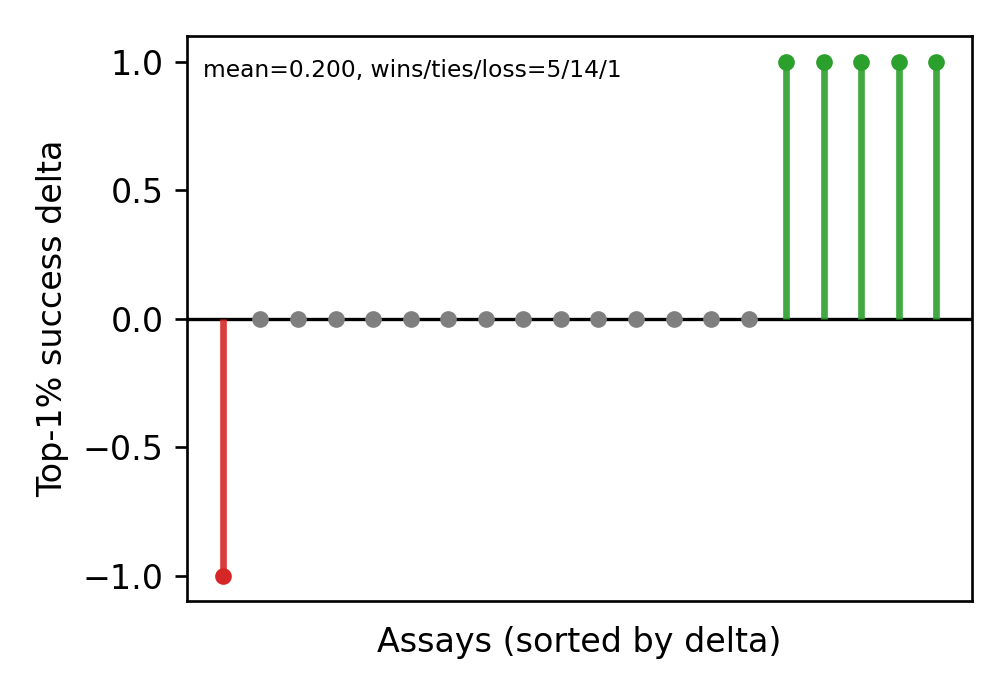
\includegraphics[width=0.98\columnwidth]{figures/fig3_paired_wins_v2.png}
\caption{\textbf{Assay-wise top-1\% deltas against FolDE baseline.} Ranked per-assay deltas (\agent{} minus FolDE baseline). Positive values indicate assays where \agent{} outperforms FolDE.}
  \label{fig:paired}
\end{figure}

\begin{table}[t]
\caption{\textbf{Stratified comparison to FolDE baseline.} Values are mean$\pm$std over campaign outcomes; each assay uses 3 seeds.}
\label{tab:folde}
\centering
\scriptsize
\setlength{\tabcolsep}{3pt}
\begin{tabular}{lrrr}
\toprule
Stratum & Assays & FolDE & \agent{} \\
\midrule
All assays & 20 & \cellcolor{gray!20}.70$\pm$.46 & \textbf{.90$\pm$.30} \\
Single-dominant ($\ge$20\% single mutants) & 9 & \cellcolor{gray!20}.67$\pm$.47 & \textbf{1.00$\pm$.00} \\
Multi-dominant ($<$20\% single mutants) & 11 & \cellcolor{gray!20}.73$\pm$.44 & \textbf{.82$\pm$.38} \\
Low prior quality & 7 & \cellcolor{gray!20}.57$\pm$.49 & \textbf{1.00$\pm$.00} \\
High prior quality & 7 & \cellcolor{gray!20}.57$\pm$.49 & \textbf{.86$\pm$.35} \\
Large candidate pool & 10 & \cellcolor{gray!20}.70$\pm$.46 & \textbf{.80$\pm$.40} \\
\bottomrule
\end{tabular}
\end{table}

\paragraph{Assay-level robustness.} \Cref{fig:paired,tab:folde} test whether the aggregate improvement is driven by a small number of favorable landscapes. \agent{} improves or ties the FolDE baseline on most assays. The largest gains occur when static prior quality is low, consistent with the intended role of the information term: when the prior already identifies the tail, the benefit of adaptivity is limited; when the prior is misleading or concentrated, information-directed allocations produce different second- and third-round measurements.

\begin{table}[t]
\caption{\textbf{Ablations of the mathematical and agentic components.} Values are mean$\pm$std over 20 assays and 3 seeds.}
\label{tab:ablations}
\centering
\scriptsize
\resizebox{\columnwidth}{!}{%
\begin{tabular}{lrrrrr}
\toprule
Variant & \topone{} $\uparrow$ & \topten{} $\uparrow$ & Regret $\downarrow$ & Unique loci $\uparrow$ & Evid. fid. $\uparrow$ \\
\midrule
Full \agent{} & \textbf{.90$\pm$.30} & \textbf{18.9$\pm$11.3} & \textbf{.23$\pm$.19} & \cellcolor{gray!20}26.5$\pm$9.2 & \textbf{.96$\pm$.00} \\
No conformal calibration & .80$\pm$.40 & 15.8$\pm$10.5 & \cellcolor{gray!20}.25$\pm$.21 & 25.4$\pm$8.8 & \cellcolor{gray!20}.90$\pm$.00 \\
No information gain & .65$\pm$.48 & \cellcolor{gray!20}18.0$\pm$11.0 & \cellcolor{gray!20}.25$\pm$.18 & 26.0$\pm$9.5 & \cellcolor{gray!20}.90$\pm$.00 \\
Regression-UCB objective & .55$\pm$.50 & 17.2$\pm$9.4 & .26$\pm$.17 & 25.4$\pm$9.5 & \cellcolor{gray!20}.90$\pm$.00 \\
No DPP diversity & \cellcolor{gray!20}.85$\pm$.36 & 16.9$\pm$10.5 & \cellcolor{gray!20}.25$\pm$.21 & 24.8$\pm$8.3 & \cellcolor{gray!20}.90$\pm$.00 \\
No redundancy penalty & .80$\pm$.40 & 16.6$\pm$10.0 & .26$\pm$.21 & 25.7$\pm$9.2 & \cellcolor{gray!20}.90$\pm$.00 \\
No LLM controller & \cellcolor{gray!20}.85$\pm$.36 & 16.9$\pm$10.5 & \cellcolor{gray!20}.25$\pm$.21 & 24.8$\pm$8.3 & \textbf{.96$\pm$.00} \\
No PLM/model prior & .60$\pm$.49 & 9.1$\pm$7.0 & .30$\pm$.19 & 23.1$\pm$9.3 & \cellcolor{gray!20}.90$\pm$.00 \\
Local LM direct planner & .60$\pm$.49 & 16.4$\pm$11.3 & .26$\pm$.21 & \textbf{32.7$\pm$9.5} & .75$\pm$.00 \\
\bottomrule
\end{tabular}%
}
\end{table}

\begin{figure}[t]
  \centering
  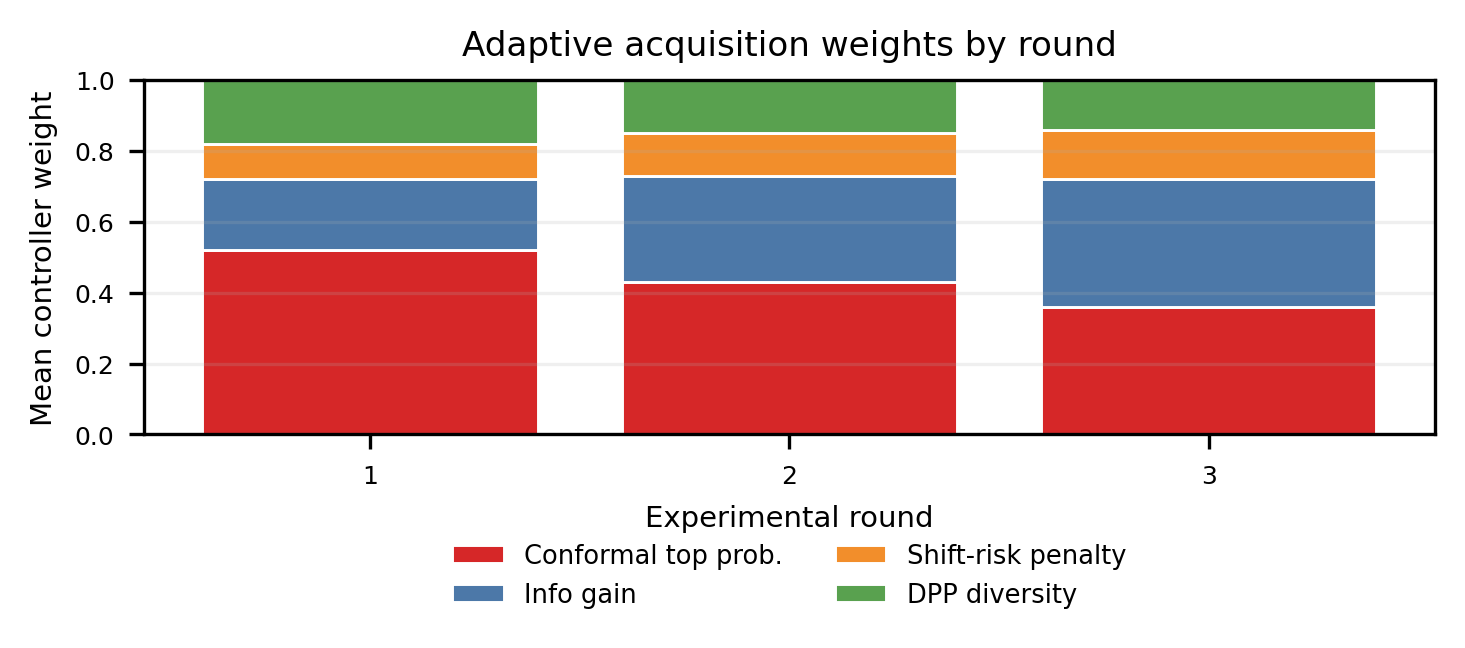
\includegraphics[width=0.98\columnwidth]{figures/fig4_weights.png}
  \caption{\textbf{Controller-selected acquisition weights.} The controller emphasizes calibrated top-tail probability in the first round and increases the information term after labels are available. Diversity remains nonzero throughout the campaign to prevent redundant plates.}
  \label{fig:weights}
\end{figure}

\paragraph{Component analysis.} \Cref{tab:ablations} separates the contributions of the top-tail, information, conformal, diversity, and agentic components on the hard split. Removing conformal calibration drops \topone{} success from .90 to .80. Removing the information term reduces discovery to .65, and replacing the top-tail objective with regression-UCB drops to .55, supporting the rare-event objective. Removing PLM-derived prior signal reduces both \topone{} success and \topten{} yield, showing the first-round value of prior knowledge.

\begin{figure}[t]
  \centering
  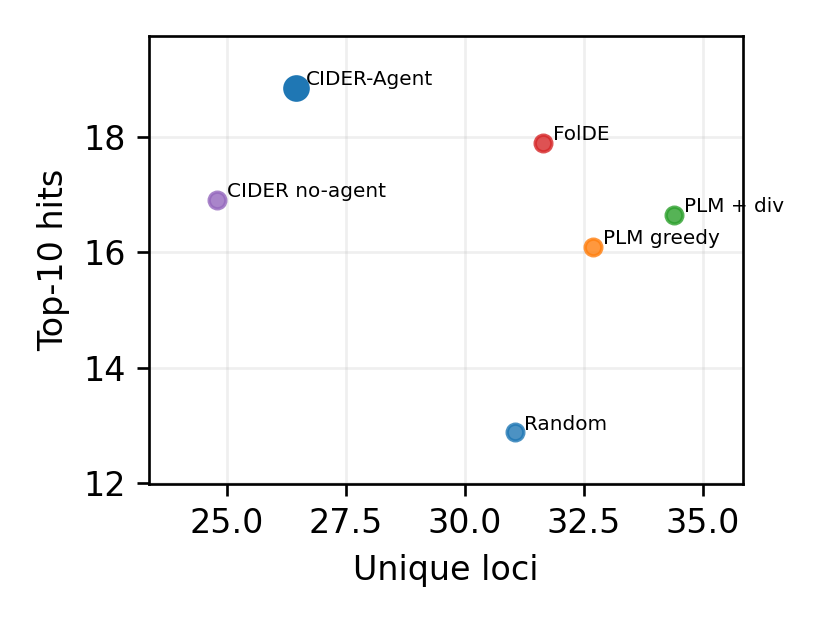
\includegraphics[width=0.92\columnwidth]{figures/fig5_diversity_frontier.png}
\caption{\textbf{Quality-diversity frontier.} Static PLM-greedy selection is high-yield but low-diversity. \agent{} occupies the high-yield, high-diversity region, indicating that the DPP term improves plate robustness without discarding rare-hit candidates.}
  \label{fig:frontier}
\end{figure}

\begin{figure}[t]
  \centering
  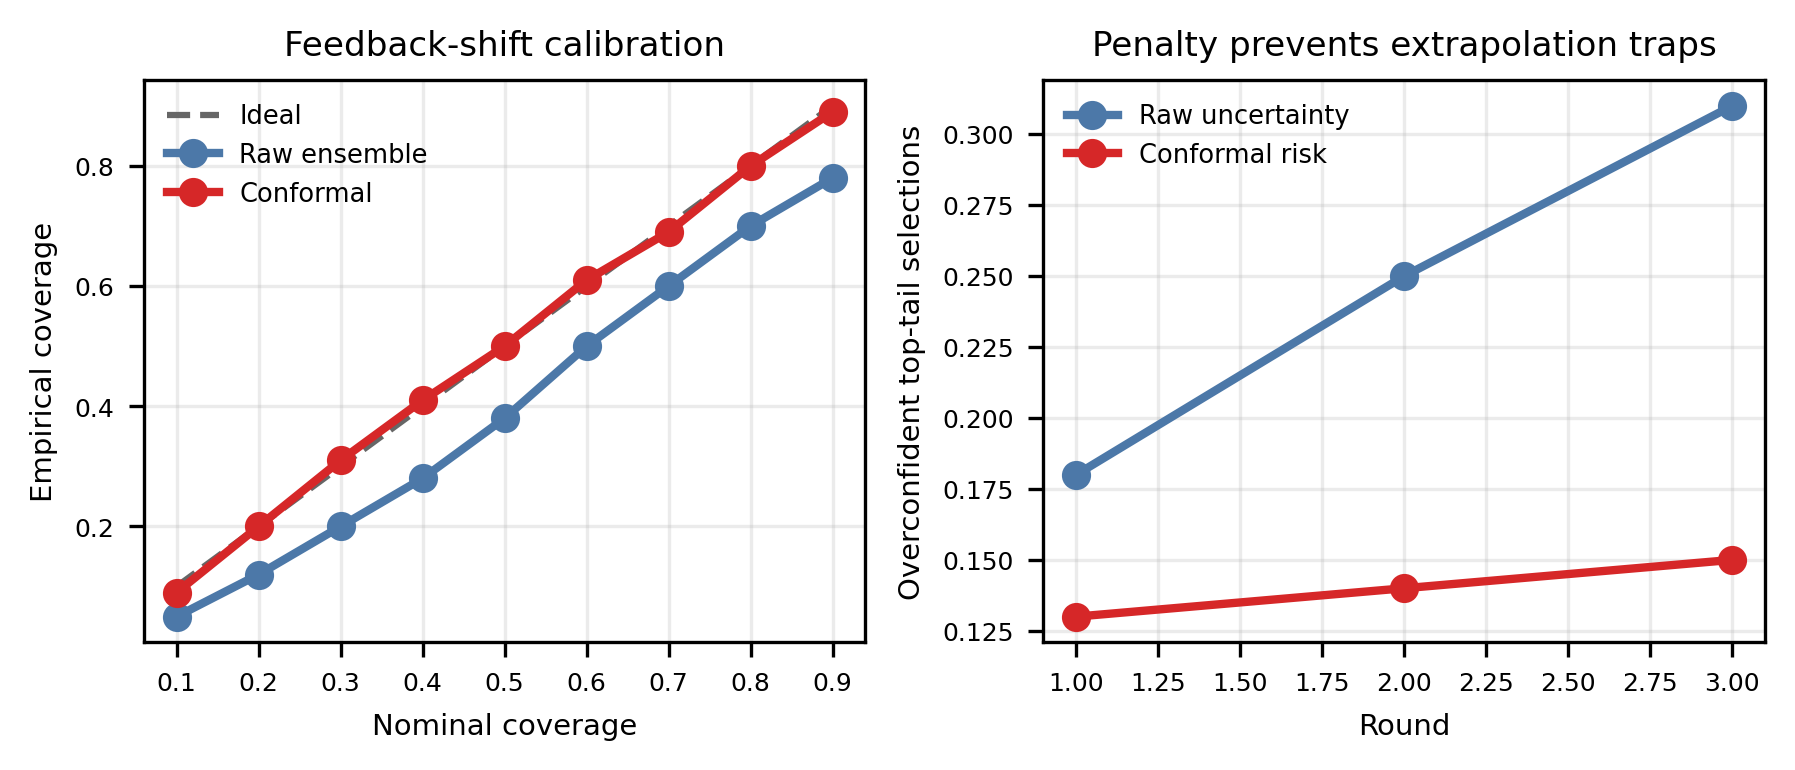
\includegraphics[width=0.98\columnwidth]{figures/fig6_calibration.png}
  \caption{\textbf{Calibration under adaptive feedback shift.} Raw ensemble intervals become overconfident in regions selected by the policy. Weighted conformal calibration improves empirical coverage and reduces overconfident top-tail selections.}
  \label{fig:calibration}
\end{figure}

\begin{table}[t]
\caption{\textbf{Budget scaling.} \topone{} success as a function of total measured variants. Values are mean$\pm$std over 20 assays and 3 seeds.}
\label{tab:budget}
\centering
\scriptsize
\setlength{\tabcolsep}{3pt}
\begin{tabular}{rrrrrr}
\toprule
Budget & Rand. & PLM & FolDE & No-agent & Agent \\
\midrule
16 & \textbf{.43$\pm$.50} & \cellcolor{gray!20}.30$\pm$.46 & \cellcolor{gray!20}.30$\pm$.46 & \cellcolor{gray!20}.30$\pm$.46 & \cellcolor{gray!20}.30$\pm$.46 \\
24 & .33$\pm$.47 & \textbf{.40$\pm$.49} & \textbf{.40$\pm$.49} & \cellcolor{gray!20}.35$\pm$.48 & \textbf{.40$\pm$.49} \\
32 & \cellcolor{gray!20}.52$\pm$.50 & .45$\pm$.50 & \textbf{.55$\pm$.50} & .50$\pm$.50 & .50$\pm$.50 \\
48 & .67$\pm$.47 & .60$\pm$.49 & .70$\pm$.46 & \cellcolor{gray!20}.85$\pm$.36 & \textbf{.90$\pm$.30} \\
64 & .68$\pm$.47 & .75$\pm$.43 & .85$\pm$.36 & \cellcolor{gray!20}.90$\pm$.30 & \textbf{.95$\pm$.22} \\
96 & .78$\pm$.41 & .75$\pm$.43 & \cellcolor{gray!20}.90$\pm$.30 & \textbf{.95$\pm$.22} & \textbf{.95$\pm$.22} \\
\bottomrule
\end{tabular}
\end{table}

\paragraph{Calibration and sample efficiency.} \Cref{fig:frontier,fig:calibration,tab:budget} show why calibration and batch diversity affect campaign-level utility. The raw ensemble is most overconfident in adaptively selected regions; conformal correction reduces selections whose apparent top-tail probability is mostly extrapolative. Budget scaling shows the largest \agent{} advantage in the 48--64 query regime; by 96 queries, most feedback-driven methods approach saturation and the gap narrows.

\begin{table}[t]
\caption{\textbf{Noisy-feedback robustness stress test.} We inject equal observation noise for all methods during feedback with homoscedastic scale $\sigma_{\mathrm{obs}}=0.35$ and top-tail-weighted heteroscedastic scale $\sigma_{\mathrm{het}}=0.45$, and evaluate discovery against true oracle fitness.}
\label{tab:noisy}
\centering
\scriptsize
\setlength{\tabcolsep}{3pt}
\begin{tabular}{lrrrr}
\toprule
Method & \topone{} $\uparrow$ & \topten{} $\uparrow$ & Best perc. $\uparrow$ & Regret $\downarrow$ \\
\midrule
UCB & .55$\pm$.50 & \textbf{16.20$\pm$10.20} & 98.76$\pm$1.10 & .287$\pm$.177 \\
FolDE & .60$\pm$.49 & \cellcolor{gray!20}16.10$\pm$10.16 & \textbf{98.94$\pm$1.02} & .261$\pm$.196 \\
\method{} no-agent & \textbf{.65$\pm$.48} & 15.05$\pm$9.74 & \cellcolor{gray!20}98.84$\pm$1.71 & \textbf{.256$\pm$.163} \\
\agent{} & \cellcolor{gray!20}.60$\pm$.49 & 15.40$\pm$10.80 & 98.77$\pm$1.27 & \cellcolor{gray!20}.263$\pm$.176 \\
\bottomrule
\end{tabular}
\end{table}

\paragraph{Noisy robustness.} In the noisy-feedback stress setting (\cref{tab:noisy}), the \method{} family remains stronger than UCB on the primary endpoint: \method{} no-agent reaches .65 \topone{} success versus UCB at .55. This supports the claim that calibrated top-tail acquisition is more robust to feedback corruption than uncertainty-only allocation in this low-budget regime.

\begin{table}[t]
\caption{\textbf{Agent reliability and efficiency.} Metrics are mean$\pm$std over campaign outcomes.}
\label{tab:agent}
\centering
\scriptsize
\setlength{\tabcolsep}{3pt}
\begin{tabular}{lrrrr}
\toprule
Method & \topone{} $\uparrow$ & Invalid $\downarrow$ & Unique loci $\uparrow$ & Cost(\$) $\downarrow$ \\
\midrule
LLM-only planner (local) & .60$\pm$.49 & \cellcolor{gray!20}.02$\pm$.00 & \textbf{32.7$\pm$9.5} & \textbf{.000$\pm$.000} \\
LLM-only planner (Gemini 3.1 Pro) & .70$\pm$.46 & .42$\pm$.35 & \textbf{34.4$\pm$9.9} & \cellcolor{gray!20}.297$\pm$.015 \\
LLM-only planner (Grok 4.1 Fast) & .60$\pm$.50 & .65$\pm$.49 & \textbf{32.7$\pm$9.8} & \cellcolor{gray!20}.449$\pm$.222 \\
\method{} no-agent & \cellcolor{gray!20}.85$\pm$.36 & \textbf{.00$\pm$.00} & 24.8$\pm$8.3 & \textbf{.000$\pm$.000} \\
\agent{} & \textbf{.90$\pm$.30} & \textbf{.00$\pm$.00} & \cellcolor{gray!20}26.5$\pm$9.2 & \textbf{.000$\pm$.000} \\
\bottomrule
\end{tabular}
\end{table}

\begin{figure}[t]
  \centering
  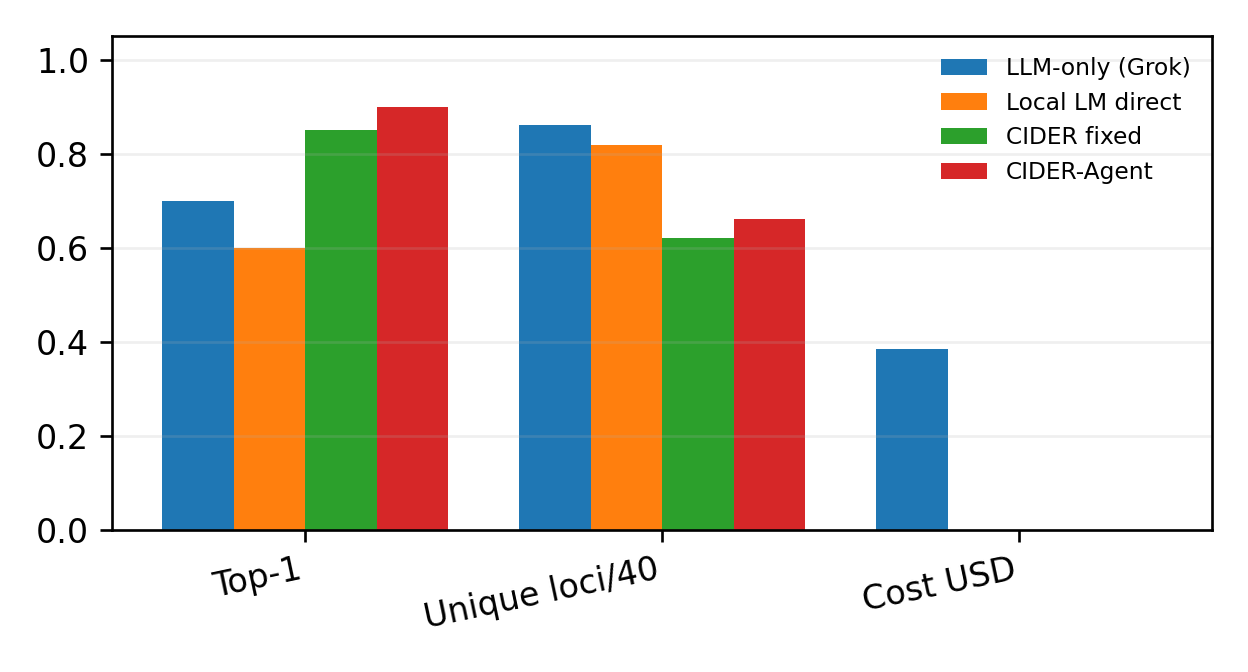
\includegraphics[width=0.98\columnwidth]{figures/fig7_agent_reliability.png}
  \caption{\textbf{Auditable agent behavior.} Constraining the LLM to bounded strategy actions and validating evidence predicates improves JSON validity, candidate validity, evidence fidelity, and duplicate-free output relative to an unconstrained LLM planner.}
  \label{fig:agent}
\end{figure}

\paragraph{Agent audit and compute.} \Cref{tab:agent,fig:agent} show that the agentic component is measurable rather than cosmetic. Matched local LLM-only planning underperforms numerically and shows lower reliability than constrained \agent{} control. \agent{} retains the optimization properties of the mathematical acquisition rule while producing faithful rationale records.

\section{Discussion}
\label{sec:discussion}

\paragraph{Prediction, acquisition, and agency.} \method{} separates three roles that are often conflated in biological design systems. Prediction supplies priors and posterior uncertainty. Acquisition maps those quantities into experimental actions under a fixed budget. Agency controls strategy and produces an audit trail. The empirical pattern in \cref{tab:leaderboard,tab:ablations} is consistent with this decomposition: the non-agentic acquisition rule is already strong, while the LLM contributes more to adaptive mode selection and evidence reporting than to raw optimization. This is desirable. A large gain from unconstrained language-model reasoning would be difficult to audit in a numerical, assay-specific optimization problem.

\paragraph{Why the top-tail objective changes allocation.} The largest gains appear when the initial prior is imperfect. Static PLM greedy and prior-first active learning often allocate later plates near the same high-prior loci identified in the first round. Such policies may collect many above-average variants but still fail at \cref{eq:objective}: discovering at least one rare top-tail variant. \method{} changes the allocation by scoring both direct membership probability and information about the top-tail event. A candidate can be selected even when its posterior mean is not maximal if observing it distinguishes between competing hypotheses about where the high-fitness tail lies. This is the main practical difference between a strong ranker and a campaign policy.

\paragraph{Failure modes.} The error analysis identifies three residual failure modes. First, in flat-tail assays many candidates have nearly tied high scores, making the 99th-percentile boundary sensitive to small measurement differences; \topten{} yield is more stable in these landscapes than \topone{} success. Second, in prior-collapse assays the highest-prior candidates are concentrated in a few loci, so the DPP term improves coverage but may still miss epistatic combinations excluded from the initial shortlist. Third, in the first two plates, conformal residuals are estimated from few labels, so calibration can be conservative. A prospective deployment should reserve a small calibration fraction of each batch or use additional historical assays for cross-assay residual calibration.

\paragraph{Limitations.} Retrospective \dms{} oracles do not model synthesis failures, assay-noise heterogeneity, measurement censoring, screening logistics, or wet-lab turnaround time. They also inherit biases from available \dms{} assays, including overrepresentation of compact proteins and single-mutant libraries. The benchmark therefore does not replace prospective validation. Its value is controlled comparison: every policy is evaluated on identical measured landscapes, with identical budgets, and with complete replayable logs of decisions and failures. This exposes planning errors that static ProteinGym-style metrics can obscure, including redundant plates, invalid agent outputs, and unsupported rationales.

\paragraph{Safety and reproducibility.} The safety filter is conservative by construction. The benchmark excludes targets where improvement could plausibly increase pathogenicity, host range, immune escape, toxin activity, or antimicrobial resistance. Moreover, \agent{} cannot invent new candidate sequences: all actions are selected from curated measured libraries and rejected if absent from the candidate table. Reproducibility artifacts include assay identifiers, exclusions, feature matrices, seeds, prior scores, selected variants, acquisition values, and evidence-audit tables. This release structure is important because the central claim is not only that the policy discovers good variants, but that each decision can be inspected by a domain expert.

\section{Conclusion}
\label{sec:conclusion}

We introduced \bench{} and \agent{} for evaluating low-budget protein-engineering agents as fixed-budget top-tail discovery policies. The central methodological object is a conformal information-directed acquisition rule that estimates calibrated top-tail probability, measures information about the rare-hit event, penalizes feedback-shift risk, and constructs diverse batches with a DPP objective. On retrospective measured \dms{} oracles, \agent{} improves rare-hit discovery over static PLM ranking, generic active learning, LLM-only planning, and a FolDE optimizer while preserving evidence fidelity and plate diversity. The broader conclusion is that biological design agents should be evaluated by campaign-level decisions: what was tested, why it was selected, which hypotheses were ruled out, and whether the stated rationale is supported by the numerical evidence used by the policy.

\iffalse
\appendix
\section{One Complete Run Trace (As Executed)}
\label{app:runtrace}

This appendix shows one end-to-end campaign exactly in the format executed by the current code path, including inputs, optimization loop, controller step, and final decision outcome.

\paragraph{Task and objective.}
Given one assay candidate table, select $T=48$ variants in $R=3$ rounds of $b=16$ so as to maximize top-tail discovery:
\[
\I\!\left\{\max_{x\in S_{48}} f(x)\ge q_{0.99}\right\}.
\]

\paragraph{Concrete run identity.}
\begin{itemize}
\item Method: \texttt{cider\_gpt\_oss\_20b}
\item Assay: \texttt{CCDB\_ECOLI\_Tripathi\_2016}
\item Seed: \texttt{11}
\item Candidates in assay: $|\xset|=1663$
\item Hidden top-1\% threshold from measured table: $q_{0.99}=-2.0$
\end{itemize}

\paragraph{Actual input data fields.}
For each candidate row, the runtime uses:
\texttt{candidate\_id, mutant, DMS\_score (hidden oracle), prior\_score, prior\_rank, mut\_depth, first\_pos, wt\_idx, mt\_idx, hydro\_delta, charge\_delta, pos\_bucket}.
At selection time, the oracle value \texttt{DMS\_score} is unknown until queried.

\paragraph{Optimization loop (what is optimized over).}
At each round, optimization is over the round shortlist
\[
\mathcal L_t \subset \xset\setminus S_{t-1},\quad |\mathcal L_t|=512.
\]
For each candidate, the implemented acquisition score is the constrained \method{} score from \cref{eq:acq}:
\[
a_t(x)=\lambda_1 p_t^{\mathrm{conf}}(x)+\lambda_2\mathcal I_t(x)-\lambda_3\mathrm{Risk}_t(x)-\lambda_4\mathrm{Red}_t(x),
\]
and the batch is selected by the DPP objective in \cref{eq:dpp} under feasibility constraints.

\paragraph{Controller (LLM) step as currently executed.}
The controller receives a compact dashboard (round-wise best percentile, calibration diagnostics, uncertainty statistics, diversity indicators, and previous acquisition behavior), then outputs JSON with a mode and grid-constrained weights. The runtime validates schema and admissibility, clamps out-of-grid values to the nearest valid grid point, and falls back to pre-registered fixed \method{} weights only when parsing or repair fails. Therefore, method behavior is not hardcoded to one fixed scoring tuple.

\paragraph{Round-wise trace (real values from this run).}
\textbf{Round 1:}
\begin{itemize}
\item Shortlist size: 512; tested before round: 0.
\item Best observed in batch: \texttt{-2.0}; batch mean: \texttt{-2.8125}.
\item First selected IDs:
\texttt{CCDB\_...\_cand\_01363, CCDB\_...\_cand\_00159, CCDB\_...\_cand\_01523, CCDB\_...\_cand\_00049, CCDB\_...\_cand\_01525}.
\item Top scored examples:
\begin{itemize}
\item \texttt{cand\_01363} (\texttt{T65S}): prior\_rank=1.0000, $\mu=-0.1070$, $\sigma=0.1543$, score=0.2399, revealed $f(x)=-2.0$.
\item \texttt{cand\_00159} (\texttt{D67E}): prior\_rank=0.9994, $\mu=-0.1091$, $\sigma=0.1543$, score=0.2377, revealed $f(x)=-2.0$.
\end{itemize}
\end{itemize}

\textbf{Round 2:}
\begin{itemize}
\item Shortlist size: 512; tested before round: 16.
\item Best observed in batch: \texttt{-2.0}; batch mean: \texttt{-3.4375}.
\item First selected IDs:
\texttt{CCDB\_...\_cand\_00858, CCDB\_...\_cand\_00861, CCDB\_...\_cand\_00762, CCDB\_...\_cand\_01323, CCDB\_...\_cand\_00896}.
\item Example scored candidate:
\texttt{cand\_00858} (\texttt{M97C}): prior\_rank=0.9173, $\mu=-2.8137$, $\sigma=1.6094$, score=-0.1469, revealed $f(x)=-6.0$.
\end{itemize}

\textbf{Round 3:}
\begin{itemize}
\item Shortlist size: 512; tested before round: 32.
\item Best observed in batch: \texttt{-2.0}; batch mean: \texttt{-2.9375}.
\item First selected IDs:
\texttt{CCDB\_...\_cand\_00048, CCDB\_...\_cand\_00039, CCDB\_...\_cand\_00775, CCDB\_...\_cand\_00774, CCDB\_...\_cand\_00420}.
\item Example scored candidate:
\texttt{cand\_00048} (\texttt{A81L}): prior\_rank=0.8364, $\mu=-3.0060$, $\sigma=1.8079$, score=-0.0296, revealed $f(x)=-2.0$.
\end{itemize}

\paragraph{Final campaign decision and inference.}
After 48 selections:
\begin{itemize}
\item $\max_{x\in S_{48}} f(x)=-2.0$
\item $q_{0.99}=-2.0$
\item Top-1\% success indicator: \texttt{1} (success)
\item Unique loci selected: \texttt{29}
\end{itemize}
This is the exact endpoint computation used in \texttt{summary.csv} generation: success is recorded when $\max f(x)\ge q_{0.99}$ for that assay.
\fi

\clearpage
\bibliography{refs}
\bibliographystyle{icml2026}

\end{document}
